% Options for packages loaded elsewhere
% Options for packages loaded elsewhere
\PassOptionsToPackage{unicode}{hyperref}
\PassOptionsToPackage{hyphens}{url}
%
\documentclass[
  10pt,
  ignorenonframetext,
  aspectratio=169,
  russian,
]{beamer}
\newif\ifbibliography
\usepackage{pgfpages}
\setbeamertemplate{caption}[numbered]
\setbeamertemplate{caption label separator}{: }
\setbeamercolor{caption name}{fg=normal text.fg}
\beamertemplatenavigationsymbolshorizontal
% remove section numbering
\setbeamertemplate{part page}{
  \centering
  \begin{beamercolorbox}[sep=16pt,center]{part title}
    \usebeamerfont{part title}\insertpart\par
  \end{beamercolorbox}
}
\setbeamertemplate{section page}{
  \centering
  \begin{beamercolorbox}[sep=12pt,center]{section title}
    \usebeamerfont{section title}\insertsection\par
  \end{beamercolorbox}
}
\setbeamertemplate{subsection page}{
  \centering
  \begin{beamercolorbox}[sep=8pt,center]{subsection title}
    \usebeamerfont{subsection title}\insertsubsection\par
  \end{beamercolorbox}
}
% Prevent slide breaks in the middle of a paragraph
\widowpenalties 1 10000
\raggedbottom
\AtBeginPart{
  \frame{\partpage}
}
\AtBeginSection{
  \ifbibliography
  \else
    \frame{\sectionpage}
  \fi
}
\AtBeginSubsection{
  \frame{\subsectionpage}
}
\usepackage{iftex}
\ifPDFTeX
  \usepackage[T1]{fontenc}
  \usepackage[utf8]{inputenc}
  \usepackage{textcomp} % provide euro and other symbols
\else % if luatex or xetex
  \usepackage{unicode-math} % this also loads fontspec
  \defaultfontfeatures{Scale=MatchLowercase}
  \defaultfontfeatures[\rmfamily]{Ligatures=TeX,Scale=1}
\fi
\usepackage{lmodern}

\usetheme[]{metropolis}
\usefonttheme{serif} % use mainfont rather than sansfont for slide text
\ifPDFTeX\else
  % xetex/luatex font selection
  \setmainfont[]{DejaVu Sans}
  \setsansfont[]{DejaVu Sans}
  \setmonofont[]{DejaVu Sans Mono}
\fi
% Use upquote if available, for straight quotes in verbatim environments
\IfFileExists{upquote.sty}{\usepackage{upquote}}{}
\IfFileExists{microtype.sty}{% use microtype if available
  \usepackage[]{microtype}
  \UseMicrotypeSet[protrusion]{basicmath} % disable protrusion for tt fonts
}{}


\usepackage{longtable,booktabs,array}
\newcounter{none} % for unnumbered tables
\usepackage{calc} % for calculating minipage widths
\usepackage{caption}
% Make caption package work with longtable
\makeatletter
\def\fnum@table{\tablename~\thetable}
\makeatother
\usepackage{graphicx}
\makeatletter
\newsavebox\pandoc@box
\newcommand*\pandocbounded[1]{% scales image to fit in text height/width
  \sbox\pandoc@box{#1}%
  \Gscale@div\@tempa{\textheight}{\dimexpr\ht\pandoc@box+\dp\pandoc@box\relax}%
  \Gscale@div\@tempb{\linewidth}{\wd\pandoc@box}%
  \ifdim\@tempb\p@<\@tempa\p@\let\@tempa\@tempb\fi% select the smaller of both
  \ifdim\@tempa\p@<\p@\scalebox{\@tempa}{\usebox\pandoc@box}%
  \else\usebox{\pandoc@box}%
  \fi%
}
% Set default figure placement to htbp
\def\fps@figure{htbp}
\makeatother



\ifLuaTeX
\usepackage[bidi=basic,shorthands=off,provide=*]{babel}
\else
\usepackage[bidi=default,shorthands=off,provide=*]{babel}
\fi
\ifPDFTeX
\else
\babelfont{rm}[]{DejaVu Sans}
\fi
\ifLuaTeX
  \usepackage{selnolig} % disable illegal ligatures
\fi


\setlength{\emergencystretch}{3em} % prevent overfull lines

\providecommand{\tightlist}{%
  \setlength{\itemsep}{0pt}\setlength{\parskip}{0pt}}



 

\usepackage[]{csquotes}

%%% Load theme
\IfFileExists{beamerthemegotham.sty}{
  %%%% Full TeXlive
  \usetheme{gotham}
  \gothamset{
    numbering=totalframenumber,
    parttocframe default=off,
    sectiontocframe default=off,
    subsectiontocframe default=off,
    tocframe template=gotham bullet,
    % progressbar position=frametitle,
    progressbar position=foot,
  }
  \renewcommand{\gothamInstituteLogoSquare}[1][4ex]{%
    
\includegraphics[height=##1]{_resources/image/logo_rudn-inverted.png}
  }
  % \renewcommand{\gothamtitlepagelogo}[1][4ex]{%
  %   
\includegraphics[height=##1]{_resources/image/logo_rudn.png}
  % }
}{%
  %%%% TinyTeX
  \usepackage{libertine}
  %%%% https://deic.uab.cat/~iblanes/beamer_gallery/
  \usetheme{Madrid}
}
\metroset{progressbar=frametitle,numbering=fraction}
\setbeamersize{text margin left=8mm,text margin right=8mm}
\makeatletter
\@ifpackageloaded{caption}{}{\usepackage{caption}}
\AtBeginDocument{%
\ifdefined\contentsname
  \renewcommand*\contentsname{Содержание}
\else
  \newcommand\contentsname{Содержание}
\fi
\ifdefined\listfigurename
  \renewcommand*\listfigurename{Список иллюстраций}
\else
  \newcommand\listfigurename{Список иллюстраций}
\fi
\ifdefined\listtablename
  \renewcommand*\listtablename{Список таблиц}
\else
  \newcommand\listtablename{Список таблиц}
\fi
\ifdefined\figurename
  \renewcommand*\figurename{Рисунок}
\else
  \newcommand\figurename{Рисунок}
\fi
\ifdefined\tablename
  \renewcommand*\tablename{Таблица}
\else
  \newcommand\tablename{Таблица}
\fi
}
\@ifpackageloaded{float}{}{\usepackage{float}}
\floatstyle{ruled}
\@ifundefined{c@chapter}{\newfloat{codelisting}{h}{lop}}{\newfloat{codelisting}{h}{lop}[chapter]}
\floatname{codelisting}{Список}
\newcommand*\listoflistings{\listof{codelisting}{Листинги}}
\makeatother
\makeatletter
\makeatother
\makeatletter
\@ifpackageloaded{caption}{}{\usepackage{caption}}
\@ifpackageloaded{subcaption}{}{\usepackage{subcaption}}
\makeatother

\usepackage{bookmark}
\IfFileExists{xurl.sty}{\usepackage{xurl}}{} % add URL line breaks if available
\urlstyle{same}
% fallback for those not using the hyperref driver hyperxmp:
\makeatletter
\@ifundefined{xmpquote}{\newcommand{\xmpquote}[1]{#1}}{}
\makeatother
\hypersetup{
  pdftitle={Лабораторная работа № 3},
  pdfauthor={Нечаева Кира Андреевна},
  pdflang={ru-RU},
  hidelinks,
  pdfcreator={LaTeX via pandoc}}


\title{\texorpdfstring{Лабораторная работа №
3}{Лабораторная работа № 3}}
\subtitle{\texorpdfstring{Агентное моделирование:
Daisyworld}{Агентное моделирование: Daisyworld}}
\author{Нечаева Кира Андреевна}
\date{}
\institute{НКНбд-01-23}

\begin{document}
\frame{\titlepage}


\begin{frame}[fragile]{Цель работы}
\protect\phantomsection\label{ux446ux435ux43bux44c-ux440ux430ux431ux43eux442ux44b}
\textbf{Цель:} реализовать и исследовать агентную модель Daisyworld
средствами Julia и \texttt{Agents.jl}.

В работе:

\begin{itemize}
\tightlist
\item
  определены агенты и правила их поведения;
\item
  реализована клеточная среда;
\item
  построена визуализация модели;
\item
  исследована численность маргариток;
\item
  проанализирована реакция на изменение светимости;
\item
  проведены параметрические эксперименты.
\end{itemize}
\end{frame}

\begin{frame}{Агентный подход}
\protect\phantomsection\label{ux430ux433ux435ux43dux442ux43dux44bux439-ux43fux43eux434ux445ux43eux434}
\begin{columns}[c]
\begin{column}{0.42\linewidth}
В агентной модели глобальная динамика не задаётся напрямую.

Она возникает из локальных действий отдельных агентов.

В Daisyworld агент --- отдельная маргаритка со свойствами:

\begin{itemize}
\tightlist
\item
  вид;
\item
  возраст;
\item
  альбедо.
\end{itemize}

Среда --- клеточная сетка с локальной температурой.
\end{column}

\begin{column}{0.58\linewidth}
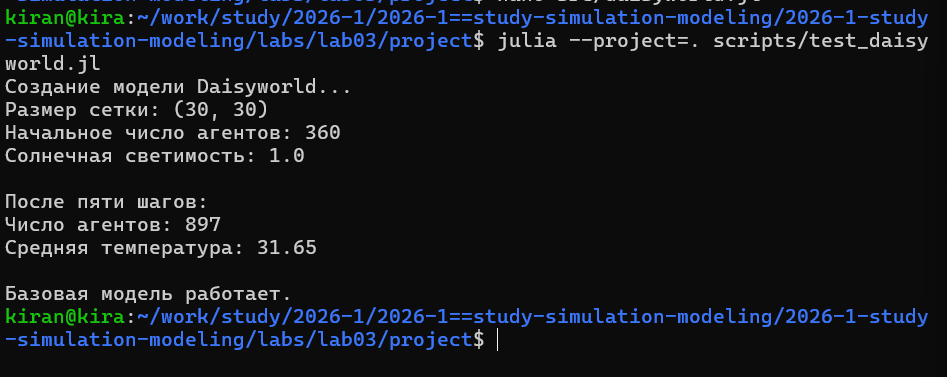
\includegraphics[width=1\linewidth,height=\textheight,keepaspectratio]{image/3.png}
\end{column}
\end{columns}
\end{frame}

\begin{frame}{Модель Daisyworld}
\protect\phantomsection\label{ux43cux43eux434ux435ux43bux44c-daisyworld}
\begin{columns}[c]
\begin{column}{0.34\linewidth}
Используются два типа агентов:

\textbf{чёрные маргаритки}

\begin{itemize}
\tightlist
\item
  меньше отражают свет;
\item
  сильнее нагревают поверхность;
\end{itemize}

\textbf{белые маргаритки}

\begin{itemize}
\tightlist
\item
  сильнее отражают свет;
\item
  охлаждают поверхность.
\end{itemize}

Температура влияет на размножение агентов.
\end{column}

\begin{column}{0.66\linewidth}
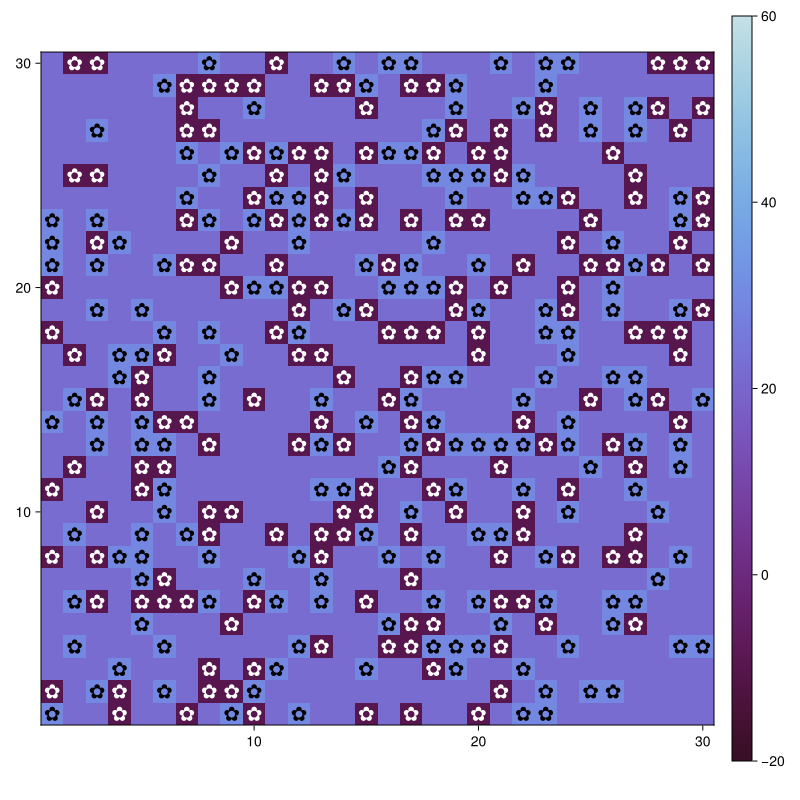
\includegraphics[width=0.88\linewidth,height=\textheight,keepaspectratio]{image/plots/daisy_step001.png}
\end{column}
\end{columns}
\end{frame}

\begin{frame}{Эволюция системы}
\protect\phantomsection\label{ux44dux432ux43eux43bux44eux446ux438ux44f-ux441ux438ux441ux442ux435ux43cux44b}
\begin{columns}[c]
\begin{column}{0.31\linewidth}
На каждом модельном шаге:

\begin{enumerate}
\tightlist
\item
  обновляется локальная температура;
\item
  температура распространяется между соседними клетками;
\item
  маргаритки могут размножаться;
\item
  агенты стареют и умирают.
\end{enumerate}

Так состояние мира изменяется без задания глобальной траектории.
\end{column}

\begin{column}{0.69\linewidth}
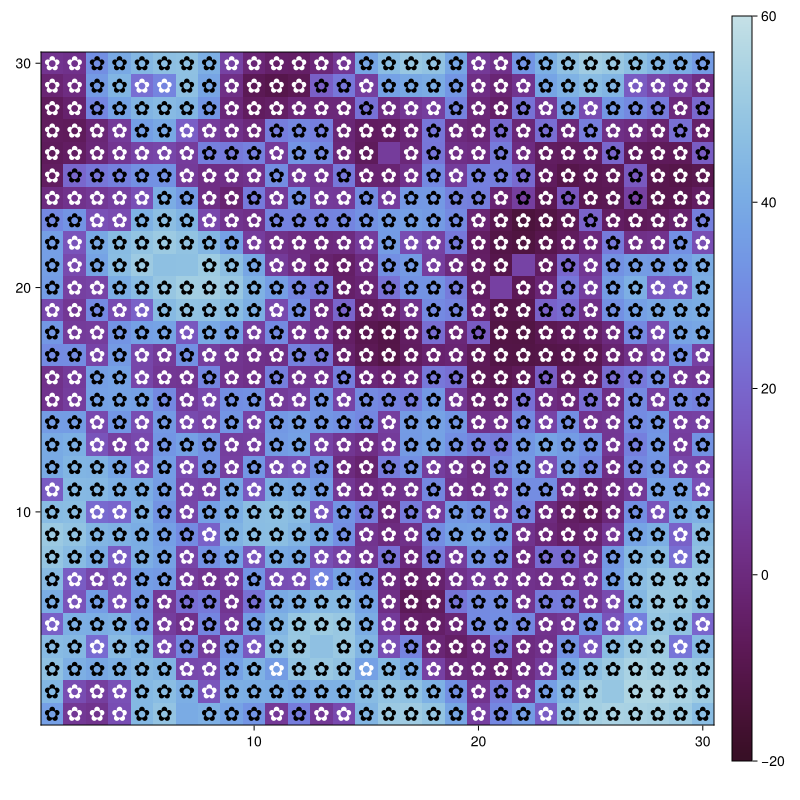
\includegraphics[width=0.88\linewidth,height=\textheight,keepaspectratio]{image/plots/daisy_step040.png}
\end{column}
\end{columns}
\end{frame}

\begin{frame}{Динамика численности}
\protect\phantomsection\label{ux434ux438ux43dux430ux43cux438ux43aux430-ux447ux438ux441ux43bux435ux43dux43dux43eux441ux442ux438}
\begin{columns}[c]
\begin{column}{0.31\linewidth}
На протяжении 1000 шагов отдельно собиралось число:

\begin{itemize}
\tightlist
\item
  чёрных маргариток;
\item
  белых маргариток.
\end{itemize}

После начального переходного процесса система формирует динамическое
состояние, поддерживаемое взаимодействием агентов и среды.
\end{column}

\begin{column}{0.69\linewidth}
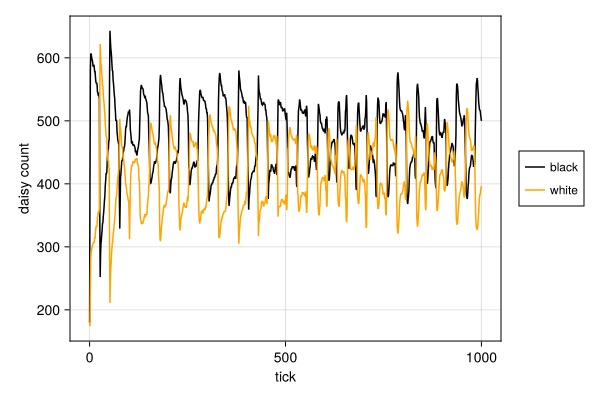
\includegraphics[width=1\linewidth,height=\textheight,keepaspectratio]{image/plots/daisy_count.png}
\end{column}
\end{columns}
\end{frame}

\begin{frame}[fragile]{Изменение солнечной светимости}
\protect\phantomsection\label{ux438ux437ux43cux435ux43dux435ux43dux438ux435-ux441ux43eux43bux43dux435ux447ux43dux43eux439-ux441ux432ux435ux442ux438ux43cux43eux441ux442ux438}
\begin{columns}[c]
\begin{column}{0.3\linewidth}
В сценарии \texttt{ramp} внешняя солнечная светимость сначала
возрастает, а затем снижается.

Одновременно собираются:

\begin{itemize}
\tightlist
\item
  численность агентов;
\item
  средняя температура;
\item
  светимость.
\end{itemize}

Это позволяет наблюдать реакцию Daisyworld на изменение внешних условий.
\end{column}

\begin{column}{0.7\linewidth}
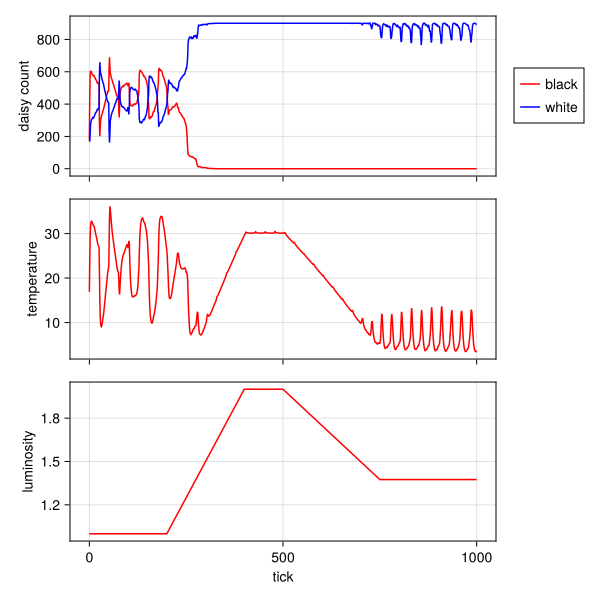
\includegraphics[width=0.92\linewidth,height=\textheight,keepaspectratio]{image/plots/daisy_luminosity.png}
\end{column}
\end{columns}
\end{frame}

\begin{frame}{Саморегуляция Daisyworld}
\protect\phantomsection\label{ux441ux430ux43cux43eux440ux435ux433ux443ux43bux44fux446ux438ux44f-daisyworld}
\begin{columns}[c]
\begin{column}{0.38\linewidth}
Связь в модели двусторонняя:

\textbf{светимость → температура → маргаритки}

и одновременно

\textbf{маргаритки → альбедо → температура}.

Поэтому изменение состава популяции влияет на климатическую среду самой
модели.
\end{column}

\begin{column}{0.62\linewidth}
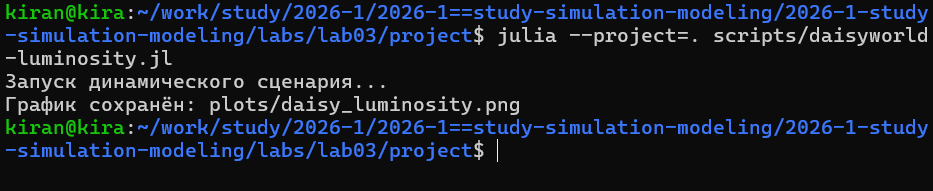
\includegraphics[width=1\linewidth,height=\textheight,keepaspectratio]{image/9.png}
\end{column}
\end{columns}
\end{frame}

\begin{frame}[fragile]{Параметрическое исследование}
\protect\phantomsection\label{ux43fux430ux440ux430ux43cux435ux442ux440ux438ux447ux435ux441ux43aux43eux435-ux438ux441ux441ux43bux435ux434ux43eux432ux430ux43dux438ux435}
\begin{columns}[c]
\begin{column}{0.31\linewidth}
В серии экспериментов изменялись:

\begin{itemize}
\tightlist
\item
  \texttt{max\_age} --- максимальный возраст агентов;
\item
  \texttt{init\_white} --- начальная доля белых маргариток.
\end{itemize}

Все комбинации создавались автоматически через \texttt{dict\_list}.
\end{column}

\begin{column}{0.69\linewidth}
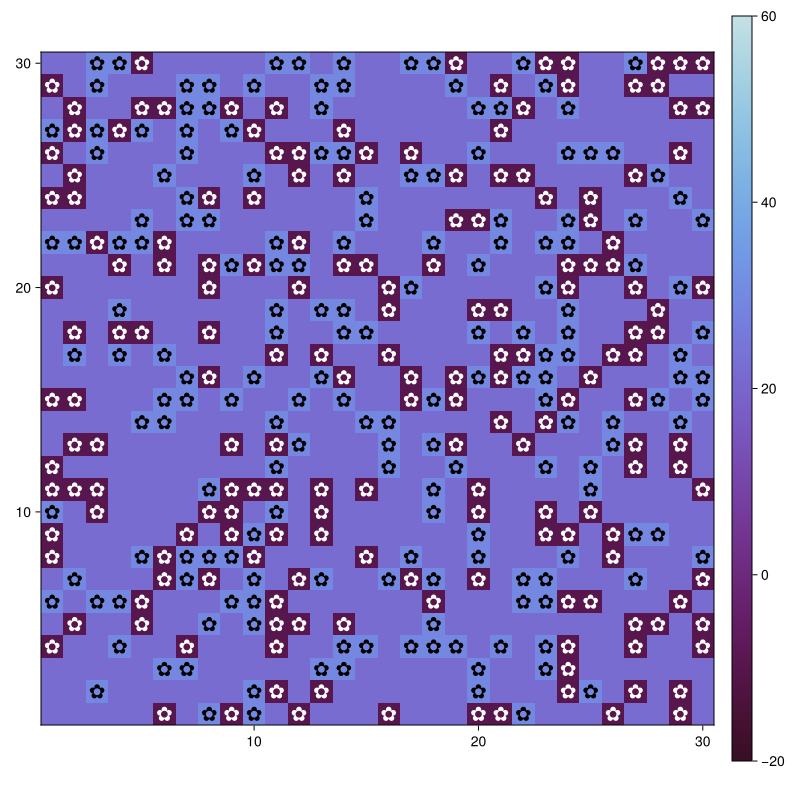
\includegraphics[width=0.88\linewidth,height=\textheight,keepaspectratio]{image/plots/params/daisyworld_param_1.png}
\end{column}
\end{columns}
\end{frame}

\begin{frame}{Сравнение параметров}
\protect\phantomsection\label{ux441ux440ux430ux432ux43dux435ux43dux438ux435-ux43fux430ux440ux430ux43cux435ux442ux440ux43eux432}
\begin{columns}[c]
\begin{column}{0.3\linewidth}
Изменение параметров меняет начальную структуру популяции и время жизни
агентов.

В результате система может выходить на разные режимы численности и
температуры.
\end{column}

\begin{column}{0.7\linewidth}
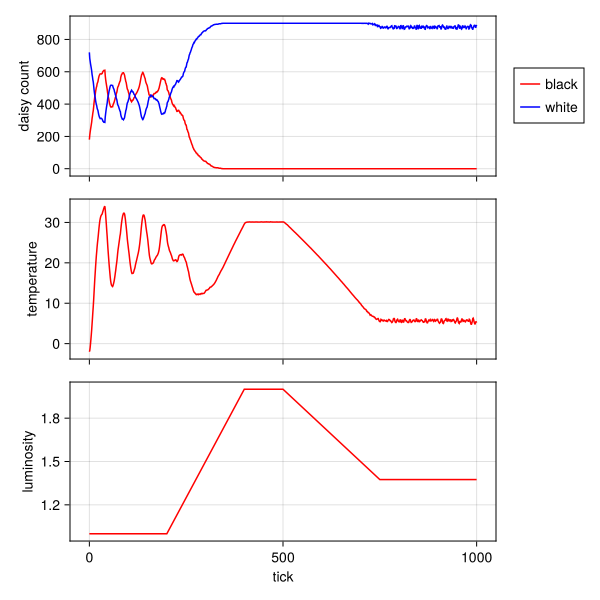
\includegraphics[width=0.92\linewidth,height=\textheight,keepaspectratio]{image/plots/params/luminosity_param_2.png}
\end{column}
\end{columns}
\end{frame}

\begin{frame}{Литературное программирование}
\protect\phantomsection\label{ux43bux438ux442ux435ux440ux430ux442ux443ux440ux43dux43eux435-ux43fux440ux43eux433ux440ux430ux43cux43cux438ux440ux43eux432ux430ux43dux438ux435}
\begin{columns}[c]
\begin{column}{0.38\linewidth}
Основные программы оформлены в литературном стиле.

Из каждого исходника автоматически создаются:

\begin{itemize}
\tightlist
\item
  чистый Julia-код;
\item
  Quarto-документация;
\item
  Jupyter Notebook.
\end{itemize}
\end{column}

\begin{column}{0.62\linewidth}
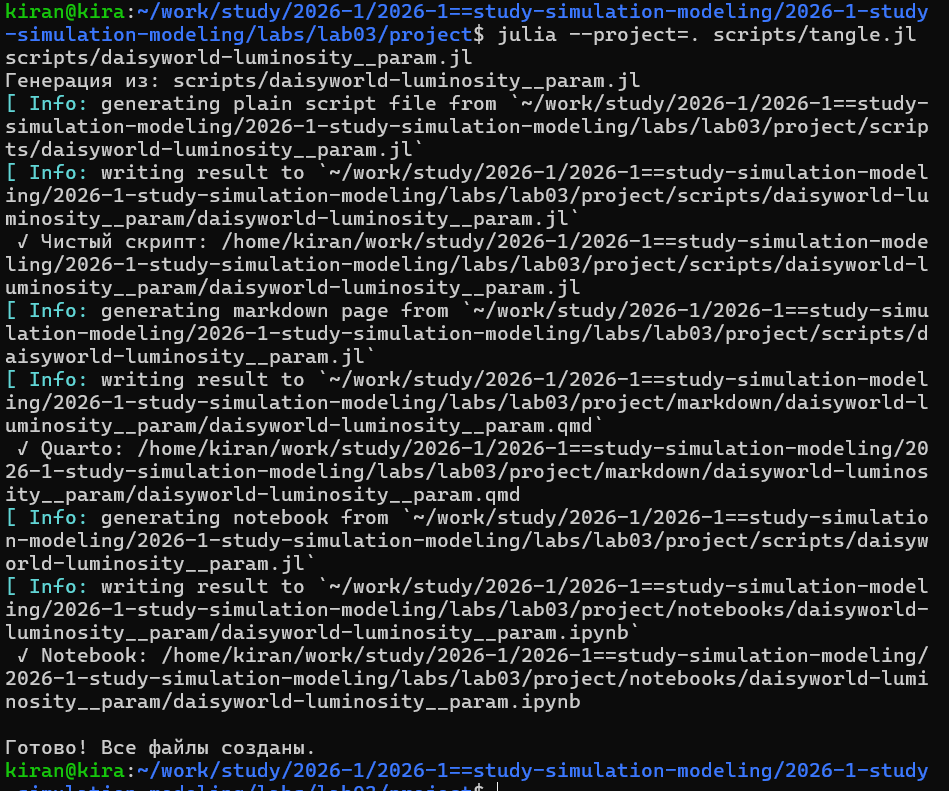
\includegraphics[width=1\linewidth,height=\textheight,keepaspectratio]{image/14.png}
\end{column}
\end{columns}
\end{frame}

\begin{frame}{Проверка воспроизводимости}
\protect\phantomsection\label{ux43fux440ux43eux432ux435ux440ux43aux430-ux432ux43eux441ux43fux440ux43eux438ux437ux432ux43eux434ux438ux43cux43eux441ux442ux438}
\begin{columns}[c]
\begin{column}{0.37\linewidth}
Все автоматически созданные notebooks были выполнены повторно.

Это проверяет, что вычислительный эксперимент можно воспроизвести не
только из исходного скрипта.
\end{column}

\begin{column}{0.63\linewidth}
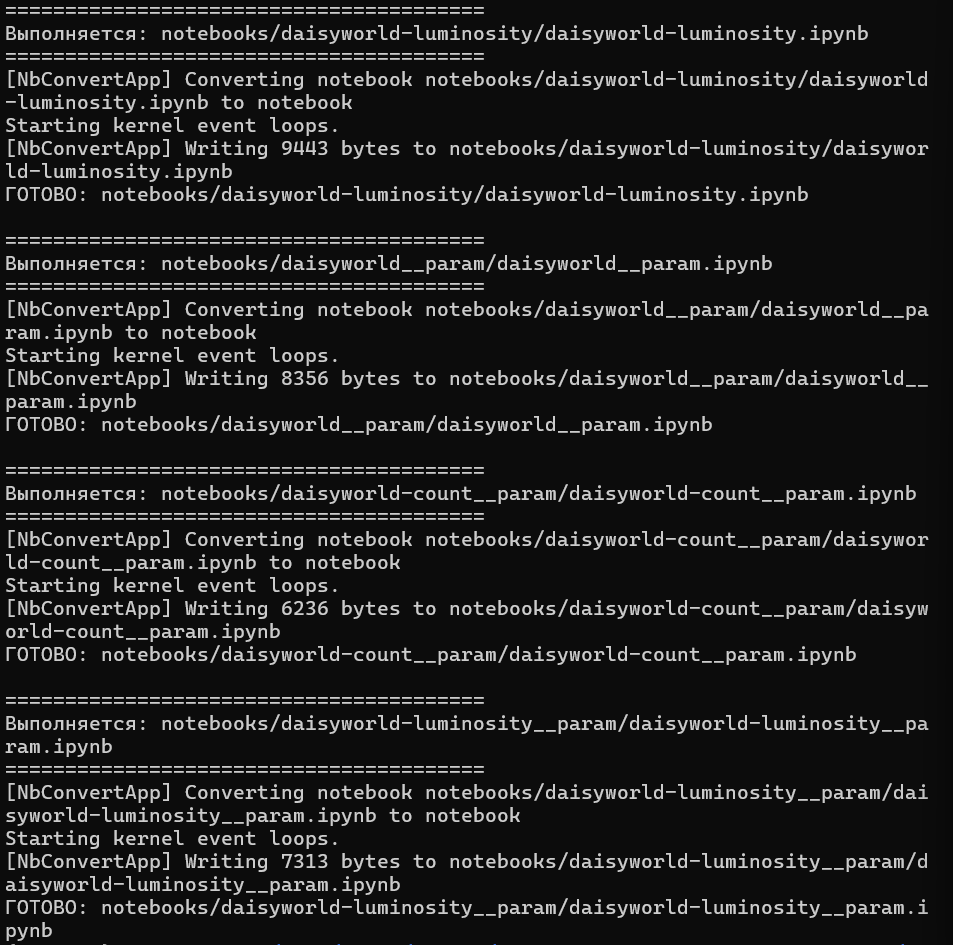
\includegraphics[width=1\linewidth,height=\textheight,keepaspectratio]{image/15.png}
\end{column}
\end{columns}
\end{frame}

\begin{frame}{Результаты разработки}
\protect\phantomsection\label{ux440ux435ux437ux443ux43bux44cux442ux430ux442ux44b-ux440ux430ux437ux440ux430ux431ux43eux442ux43aux438}
\begin{columns}[c]
\begin{column}{0.39\linewidth}
В проекте сохранены:

\begin{itemize}
\tightlist
\item
  ядро модели;
\item
  программы экспериментов;
\item
  Quarto-документация;
\item
  notebooks;
\item
  статические визуализации;
\item
  параметрические результаты;
\item
  анимация Daisyworld.
\end{itemize}
\end{column}

\begin{column}{0.61\linewidth}
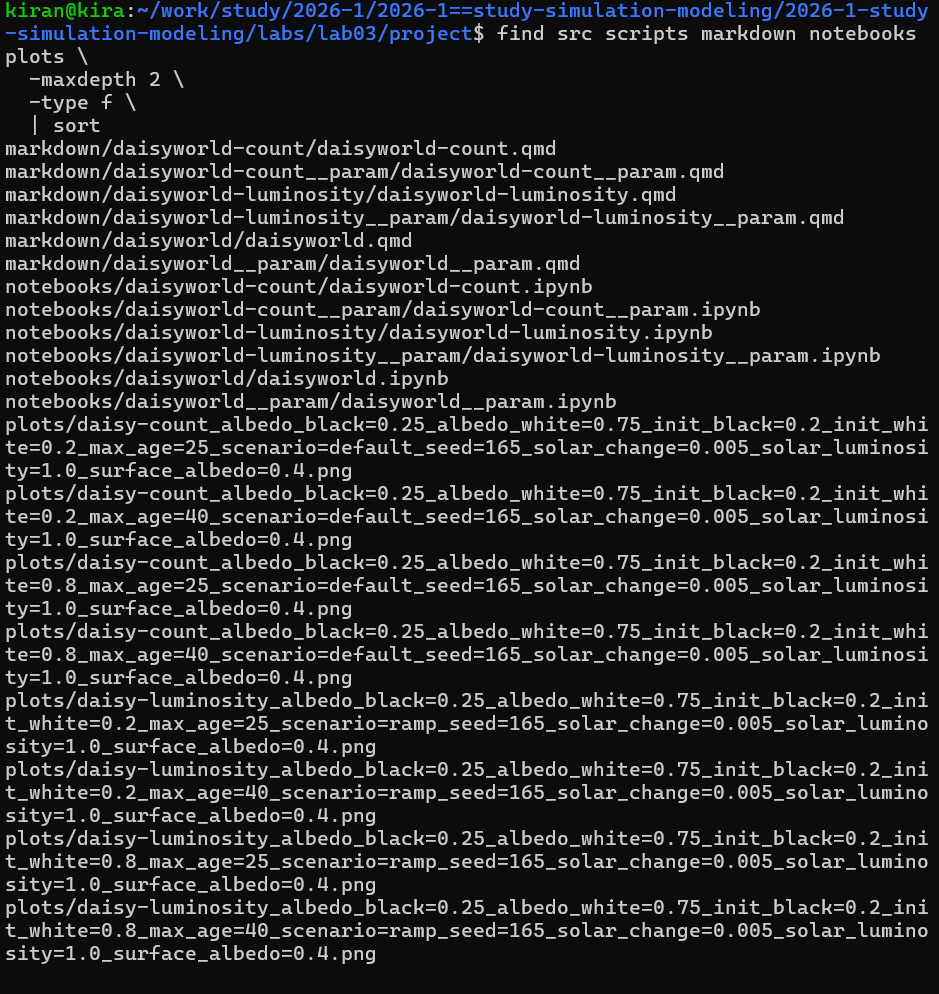
\includegraphics[width=1\linewidth,height=\textheight,keepaspectratio]{image/16.png}
\end{column}
\end{columns}
\end{frame}

\begin{frame}{Выводы}
\protect\phantomsection\label{ux432ux44bux432ux43eux434ux44b}
В лабораторной работе реализована агентная модель Daisyworld.

\begin{itemize}
\tightlist
\item
  глобальная динамика возникает из локальных действий агентов;
\item
  маргаритки и температура образуют систему с обратной связью;
\item
  модель реагирует на изменение солнечной светимости;
\item
  параметры агентов влияют на режим работы системы;
\item
  все эксперименты оформлены как воспроизводимый Julia-проект.
\end{itemize}

\textbf{Исходный код, результаты и документация сохранены программно.}
\end{frame}




\end{document}
